%% LyX 2.0.8.1 created this file.  For more info, see http://www.lyx.org/.
%% Do not edit unless you really know what you are doing.
\documentclass{article}
\usepackage[latin9]{inputenc}
\usepackage{listings}
\setlength{\parskip}{\medskipamount}
\setlength{\parindent}{0pt}
\usepackage{float}
\usepackage{amsmath}
\usepackage{amssymb}
\usepackage{graphicx}

\makeatletter

%%%%%%%%%%%%%%%%%%%%%%%%%%%%%% LyX specific LaTeX commands.
\floatstyle{ruled}
\newfloat{algorithm}{tbp}{loa}
\providecommand{\algorithmname}{Algorithm}
\floatname{algorithm}{\protect\algorithmname}

%%%%%%%%%%%%%%%%%%%%%%%%%%%%%% User specified LaTeX commands.

%
\usepackage{amsfonts}
%\usepackage{mathabx}
\usepackage{nopageno}%%%  The following few lines affect the margin sizes. 
\usepackage{bm}
\addtolength{\topmargin}{-.5in}
\setlength{\textwidth}{6in}       
\setlength{\oddsidemargin}{.25in}              
\setlength{\evensidemargin}{.25in}         
  
\setlength{\textheight}{9in}
\renewcommand{\baselinestretch}{1}
\reversemarginpar   
%
%
% Added by lyx2lyx
\usepackage{cancel}
% Added by lyx2lyx
\usepackage{mathtools}
\usepackage{tikz}
\usetikzlibrary{arrows,backgrounds,calc,trees,positioning}

\pgfdeclarelayer{background}
\pgfsetlayers{background,main}


\newcommand{\convexpath}[2]{
[   
    create hullnodes/.code={
        \global\edef\namelist{#1}
        \foreach [count=\counter] \nodename in \namelist {
            \global\edef\numberofnodes{\counter}
            \node at (\nodename) [draw=none,name=hullnode\counter] {};
        }
        \node at (hullnode\numberofnodes) [name=hullnode0,draw=none] {};
        \pgfmathtruncatemacro\lastnumber{\numberofnodes+1}
        \node at (hullnode1) [name=hullnode\lastnumber,draw=none] {};
    },
    create hullnodes
]
($(hullnode1)!#2!-90:(hullnode0)$)
\foreach [
    evaluate=\currentnode as \previousnode using \currentnode-1,
    evaluate=\currentnode as \nextnode using \currentnode+1
    ] \currentnode in {1,...,\numberofnodes} {
-- ($(hullnode\currentnode)!#2!-90:(hullnode\previousnode)$)
  let \p1 = ($(hullnode\currentnode)!#2!-90:(hullnode\previousnode) - (hullnode\currentnode)$),
    \n1 = {atan2(\x1,\y1)},
    \p2 = ($(hullnode\currentnode)!#2!90:(hullnode\nextnode) - (hullnode\currentnode)$),
    \n2 = {atan2(\x2,\y2)},
    \n{delta} = {-Mod(\n1-\n2,360)}
  in 
    {arc [start angle=\n1, delta angle=\n{delta}, radius=#2]}
}
-- cycle
}

\makeatother

\begin{document}

\title{Tarjan's least common ancestor}

\maketitle
This took me a little while to figure out. Let's start out with a
related problem: range-minimum query%
\footnote{I stole most of this from http://wcipeg.com/wiki/Lowest\_common\_ancestor\#Properties%
}. Consider the tree 
\begin{figure}[H]
\noindent \begin{centering}
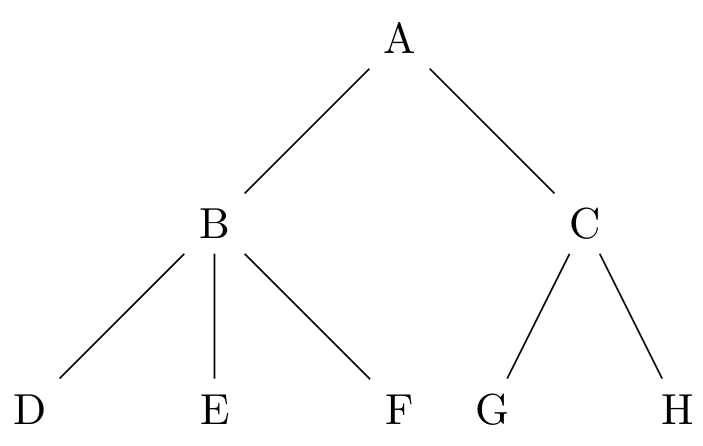
\includegraphics[scale=0.3]{Lca_example_tree}\caption{Example tree}

\par\end{centering}

\end{figure}


You can build an array with property that the least common ancestor
of any two nodes in the tree can be determind by finding the minimum
of some related range in the array. For example suppose the corresponding
array to the example tree is 
\[
T=\left[0,1,2,1,2,1,2,1,0,1,2,1,2,1,0\right]
\]
where the element-wise correspondence is 
\[
T'=\left[A,B,D,B,E,B,F,B,A,C,G,C,H,C,A\right]
\]
Then the least common ancestor (LCA) of any two nodes $u,v$ in $T'$
is the node corresponding to the minimum of the range in $T'$ corresponding
to$\left[u,v\right]$. For example $LCA\left(\left\{ D,F\right\} \right)=\min\left(\left[2,1,2\right]\right)=1=B$.
This looks purely coincidental and hinky but it's true. Try it for
any pair of nodes. It's not coincidental because of how $T$ was constructed%
\footnote{Also notice that $T'$ is the depth of the nodes in the tree.%
} from the example tree: it's an Euler circuit of the corresponding
digraph%
\footnote{A traversal of the tree that starts and ends at the same node, and
visits every edge exactly once (the digraph corresponding to the tree
has two edges for every edge in the undirected tree).%
} to the tree. Constructing it was easy: pre-order walk but print when
you come back up to the root too:

\begin{algorithm}[H]
\begin{lstlisting}[language=Python,mathescape=true,showstringspaces=false]
Euler-Circuit($u$)
    print $u$
    for $v$ of $u$
        Euler-Circuit($v$)
        print $u$

Euler-Circuit($A$)
\end{lstlisting}


\caption{Euler circuit}
\end{algorithm}
Here's an example of how it looks on another tree
\begin{figure}[H]
\noindent \centering{}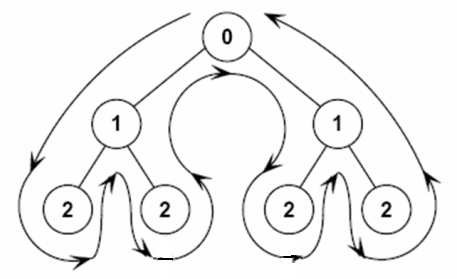
\includegraphics[scale=0.5]{euler}\caption{Example Euler circuit}
\end{figure}
Every time the traversal passes by a node it prints. The output is
$0121210121210$. 

The Euler circuit has the property that between visiting $u$ and
$v$ the $LCA\left(\left\{ u,v\right\} \right)$ is guaranteed to
be visited at least once, and no other node with depth less than or
equal to that of $LCA\left(\left\{ u,v\right\} \right)$ will appear
at all. For example, consider the nodes $D$ and $F$ in $T'$: just
like $1\in T$, node $B$ appears at least once and no shallower node
appears. Think about it: you get ``stuck'' under the least common
ancestor of $u,v$. Fact: since a tree with $n$ nodes has $n-1$
edges and the Euler circuit walks each one in the digraph corresponding
to the tree, it has length $2n-2$ and visits $2n-1$ nodes. 

Okay how do we use this to compute least common ancestor? Here is
Tarjan's least common ancestor algorithm that uses Union-Find data
structures: 
\begin{algorithm}[H]
\begin{lstlisting}[language=Python,mathescape=true,showstringspaces=false,tabsize=4]
global P // set of pairs you want to find common ancestors for

for $u$ in Tree:
	$u.color$ := BLUE

LCA($u$)
	Make-Set($u$)
	Find-Set($u$).ancestor := $u$
	for each child of $v$ of $u$
		LCA($v$)
		Union($u,v$)
		Find-Set($u$).ancestor := $u$
	$u.color$ := RED
	for each $v$ such that $\{u,v\} \in P$  
		if $v.color ==$  RED
			print "LCA($\{u,v\}$) is: " Find-Set($v$).ancestor
\end{lstlisting}


\caption{Tarjan's algorithm}
\end{algorithm}
Notice the similarity to \texttt{Euler-Circuit. }The algorithm proceeds
growing ``bottom up'' sets corresponding to subtrees whose roots
are the least common ancestor of any pair of nodes in the tree\textbf{
which have been completely traversed by the Euler circuit}, i.e. colord
\texttt{RED}. A picture is worth a thousand words so here are bunch:
I'll walk through the operation of the algorithm if $P$ is every
pair of nodes in the Example tree.
\begin{enumerate}
\item 
\item 
\begin{figure}[H]
\noindent \centering{}\begin{tikzpicture} 
[ 
style0/.style={circle,draw=none,text centered, anchor=north, text=blue, text opacity=1}, 
style1/.style={circle,draw,fill=red,text centered,anchor=north, text=black, text opacity=1}, style2/.style={circle, draw, fill=red,fill opacity=0.3, text centered, anchor=north, text=black, text opacity=1, radius=3cm}, 
style3/.style={circle, draw=none, fill=blue,fill opacity=0.3, text centered, anchor=north, text=black, text opacity=1}, 
style4/.style={circle, draw=none, fill=green,fill opacity=0.3, text centered, anchor=north, text=black, text opacity=1}, 	
level distance=1.5cm,   
level 1/.style={sibling distance=3cm},   
level 2/.style={sibling distance=1.5cm}   
] 

\node  (A) [style2,style0] {A}
    child { node (B) [style0] {B}
			node (BB) at ($(B)!0.5!(B)$) {BB}			
       child { node (D) [style0] {D}
    }
      child { node (E) [style0] {E}
    } child { node (F) [style0] {F}
    }
  }
    child { node (C) [style0] {C}
      child { node (G) [style0] {G}
    } child { node (H) [style0] {H}
    }
  };
\begin{pgfonlayer}{background} 
%\fill[red,opacity=0.3] \convexpath{D,B,A,C,H,G,F,E}{10pt}; 
%\fill[blue,opacity=0.3] \convexpath{G,C,H}{10pt}; 
\end{pgfonlayer} \end{tikzpicture}
\end{figure}
\end{enumerate}

\end{document}
